\documentclass[fiche]{classe-tex3R}
\usepackage{style-tex3R}

\definirniveau{texte}
\definirchapitre{nil}{nom}


\begin{luacode}
    Type = 'fiche' -- 'activite' ; 'bilan' ; 'corrige' ; 'cours' ; 'DM' ; 'DS' ; 'flash' ; 'interro' ; 'TD'
    Impression = false
    Header = true -- false
    Taille = '14pt' -- nil
    Stretch = false -- false

    Correction = true -- false
    Enonce = true -- false
    Visible = true -- false

    Competence = true -- false
    Bareme = true -- false
    Difficulte = true -- false
    Source = true -- false
    Theme = true -- false
\end{luacode}
\parametrage

\begin{document}
%%%% Titre perso %%%%
\ihead{{\bfseries\LARGE\logoactif~ \underLine{\textbf{TD}~|~\mdseries Tableur\hfill {\large Licence}}\par}}

%%% Signature %%%
\iffiche\ofoot{\ccbyncsaeu\\\vspace{-0.2em}\tiny mon.mail@ac-dijon.fr}\fi

\iffiche\cfoot{\pagemark}\fi

Document test snippetview
avec classe et style branche crombez
 
\begin{itemize}
    \item format : fiche
    \item titre perso
    \item signature
    \item numéros pages
\end{itemize}

\mdseries

\subsection{Police}
\textbf{gras}, \textit{italique}, \underline{souligne}, \st{barré}, \textcolor{Red}{rouge}, \textcolor{Green}{vert}, \textcolor{Blue}{bleu}

\sethlcolor{yellow}
\hl{probleme command important utilisation sethcolor et hl}

{\tailletexte{4} probleme command tailletexte ici 4}

\subsection{Paragraphe}

\subsubsection{classique}

\begin{center}
    centrer
\end{center}

\begin{flushright}
    droite
\end{flushright}


\adjustbox{valign=t}{\begin{minipage}{0.48\linewidth}%
    minipage gauche
    \begin{itemize}
        \item item1
        \item item2
    \end{itemize}
\end{minipage}}\hfill%
\adjustbox{valign=t}{\begin{minipage}{0.48\linewidth}%
    minipage droite
    \begin{enumerate}
        \item enum1
        \item enum2
    \end{enumerate}
\end{minipage}}%






\begin{tcolorbox}
    encadrer
\end{tcolorbox}

\subsubsection{TeX3R}

\begin{visible}[true]
    texte à cacher avec trame                    
\end{visible}
\begin{visible}[false]
     Texte alternatif
\end{visible}


%%%% DÉFINITION %%%%
\begin{definition}
    def
\end{definition}

%%%% PROPRIETE %%%%
\begin{propriete}
    prop
\end{propriete}

%%%% MÉTHODE %%%%
\begin{methode}
    methode
\end{methode}

%%%% APPLICATION %%%%
\begin{application}
    app
\end{application}

Problème avec exercice

\sautligne 
(test saut ligne)
\sautdeligne
% %%%% EXERCICE %%%%
% \begin{exercice}
%     exo
% \end{exercice}

%%%% CORRECTION %%%%
\begin{correction}
    Correction apres exercice (manque parametre pour changer titre)
\end{correction}

%%%% EXEMPLE %%%%
\begin{exemple}
    exemple
\end{exemple}

%%%% REMARQUE %%%%
\begin{remarque}
    remarque
\end{remarque}

%%%% PREUVE %%%%
\begin{preuve}[test param preuve]
    preuve
\end{preuve}

%%%% ÉNONCÉ %%%%
\source{source}
\theme{ttheme1, theme2}
\competence{competence1, competence2}
\difficulte{3}

\begin{enonce}
    enonce
\end{enonce}

%%%% CORRECTION %%%%
\begin{correction}
    correction apres enonce
\end{correction}

\sautfiche
(test sautfiche)
\subsection{Insertion}

\begin{tabular}{|c|c|}%l|c|r|p{1cm}
    \hline
    \rowcolor{gray} Cellule 1 & Cellule 2\\ 
    \hline
    \cellcolor{gray} Cellule 3 & Cellule 4\\ 
    \hline
\end{tabular}

\sautligne
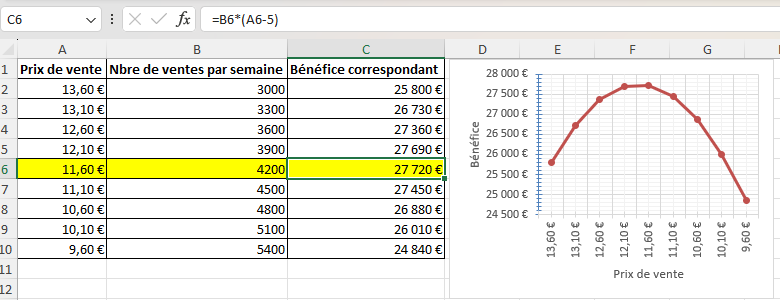
\includegraphics[width=0.6\linewidth]{image.png}

\sautligne
\begin{tikzpicture}[scale=0.5] %Echelle de la figure

    % Définition des points
    \coordinate (A) at (0,0);
    \draw (A) node[below left] {$A$}; %Etiquette haut gauche
    
    \coordinate (B) at (7,0);
    \draw (B) node[above right] {$B$}; %Etiquette bas droit
   
    \coordinate (C) at (0,3);
    \draw ($(C)+(-0.5,0.5)$) node{$C$};%Etiquette décalage manuel

     
    % Dessin du triangle
    \draw (A) -- (B) -- (C) -- cycle;
  
    % Marquage de l'angles droits
    \draw (A) rectangle ++(0.5,0.5);

      % Ajout des mesures et côtes avec décalage manuel par rapport aux sommets
    \draw[<->] ($(A)+(-0.5,0)$) -- node[left] {$AC$} ($(C)+(-0.5,0)$);
    \draw[<->] ($(A)+(0,-0.5)$) -- node[below] {$AB$} ($(B)+(0,-0.5)$);
    \draw[<->] ($(B)+(0,0.5)$) -- node[above right] {$BC$} ($(C)+(0,0.5)$);
 
\end{tikzpicture}

\sautligne
\begin{scratch}
    \blockinit{quand \greenflag est cliqué}
    \blockrepeat{répéter \ovalnum{4} fois}
    {
        \blockifelse{si \booloperator{\ovalvariable{x} > \ovalnum{1}} alors}
            {
                \blockmove{tourner de \turnleft{} de \ovalnum{45} degrés}
            }
            {
                \blockvariable{mettre \selectmenu{ma_variable} à \ovaloperator{\ovalvariable{x} + \ovalnum{10}}}
            }
    }
    \blocklook{dire \ovalnum{fin}}
\end{scratch}

\sautligne

\tracelignes{2}

\sautligne

\tracecarreaux{2}

\subsection{Math mode}
$3^{4}, 8 _{5}, \sqrt{17}, 14^\circ, \widehat{\mathrm{ABC}}, \overparen{\mathrm{ABC}}, \dfrac{3\times \cancel{4}}{\cancel{4} \times 5}, \np[km]{3450}, \ne, \approx, \times, \div, \left(tr\right),\longmapsto,\mathcal{A}, \leq,\geq$

\subsection{Autre}
\og É Ê À Ç \fg



\end{document}